\begin{comment}
\documentclass[10pt]{article}
\usepackage{fullpage, graphicx, url}
\setlength{\parskip}{1ex}
\setlength{\parindent}{0ex}
\title{GEN03}
\begin{document}


\begin{tabular}{ccc}
The Alternative Csound Reference Manual & & \\
Previous & &Next

\end{tabular}

%\hline 
\end{comment}
\section{GEN03}
GEN03�--� Generates a stored function table by evaluating a polynomial. \subsection*{Description}


  This subroutine generates a stored function table by evaluating a polynomial in x over a fixed interval and with specified coefficients. 
\subsection*{Syntax}


 \textbf{f}
 \# time size 3 xval1 xval2 c0 c1 c2 ... cn
\subsection*{Initialization}


 \emph{size }
 -- number of points in the table. Must be a power of 2 or a power-of-2 plus 1. 


 \emph{xval1, xval2 }
 -- left and right values of the x interval over which the polynomial is defined (\emph{xval1}
 $<$ \emph{xval2}
). These will produce the 1st stored value and the (power-of-2 plus l)th stored value respectively in the generated function table. 


 \emph{c0, c1, c2, ... cn}
 -- coefficients of the nth-order polynomial 


 \emph{c0 + c1x + c2x2 + . . . + cnxn}



  Coefficients may be positive or negative real numbers; a zero denotes a missing term in the polynomial. The coefficient list begins in p7, providing a current upper limit of 144 terms. 


 


\begin{tabular}{cc}
\textbf{Note}
 \\
� &

 


 
\begin{itemize}
\item 

  The defined segment [fn(\emph{xval1}
), fn(\emph{xval2}
)] is evenly distributed. Thus a 512-point table over the interval [-1,1] will have its origin at location 257 (at the start of the 2nd half). Provided the extended guard point is requested, both fn(-1) and fn(1) will exist in the table. 

\item 

 \emph{GEN03}
 is useful in conjunction with \emph{table}
 or \emph{tablei}
 for audio waveshaping (sound modification by non-linear distortion). Coefficients to produce a particular formant from a sinusoidal lookup index of known amplitude can be determined at preprocessing time using algorithms such as Chebyshev formulae. See also \emph{GEN13}
. 


\end{itemize}


\end{tabular}

\subsection*{Examples}


  Here is a simple example of the GEN03 routine. It uses the files \emph{gen03.orc}
 and \emph{gen03.sco}
. It fills a table with a 4th order polynomial function over the x-interval -1 to 1. The origin will be at the offset position 512. The function is post-normalized. Here is its diagram: 


 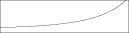
\includegraphics[scale=1]{gen03} 


 Diagram of the waveform generated by GEN03.


 \textbf{Example 1. A simple example of the GEN03 routine.}

\begin{lstlisting}
/* gen03.orc */
; Initialize the global variables.
sr = 44100
kr = 4410
ksmps = 10
nchnls = 1

; Instrument #1.
instr 1
  ; Create an index over the length of our entire note.
  kcps init 1/p3
  kndx phasor kcps

  ; Read Table #1 with our index.
  ifn = 1
  ixmode = 1
  kamp table kndx, ifn, ixmode

  ; Create a sine wave, use the Table #1 values to control
  ; the amplitude.
  a1 oscil kamp*30000, 440, 2
  out a1
endin
/* gen03.orc */
        
\end{lstlisting}
\begin{lstlisting}
/* gen03.sco */
; Table #1: a polynomial function (using GEN03).
f 1 0 1025 3 -1 1 5 4 3 2 2 1
; Table #2, a sine wave.
f 2 0 16384 10 1

; Play Instrument #1 for 2 seconds.
i 1 0 2
e
/* gen03.sco */
        
\end{lstlisting}
\subsection*{See Also}


 \emph{GEN13}
, \emph{GEN14}
, and \emph{GEN15}
. 
%\hline 


\begin{comment}
\begin{tabular}{lcr}
Previous &Home &Next \\
GEN02 &Up &GEN04

\end{tabular}


\end{document}
\end{comment}
